\chapter{Methodik}
\label{chap:methodik}

In diesem Kapitel wird der methodische Aufbau dieser Thesis beschrieben und begründet.
Die Arbeit ist als industrielle Fallstudie in Zusammenarbeit mit \emph{levigo solutions} konzipiert und dient der Evaluation des \gls{mmf} an einer bestehenden Microservices-Architektur.
Diese Fallstudie besteht aus zwei Hauptbestandteilen.
Im ersten Teil wird ein Refactoring des Produktes \emph{jadice flow} nach Anleitung des Frameworks durchgeführt.
Im zweiten Teil wird das Ergebnis dieses Refactorings verwendet, um eine Evaluation des Frameworks und Tools abzuschließen.

\begin{figure}[!ht]
	\centering
	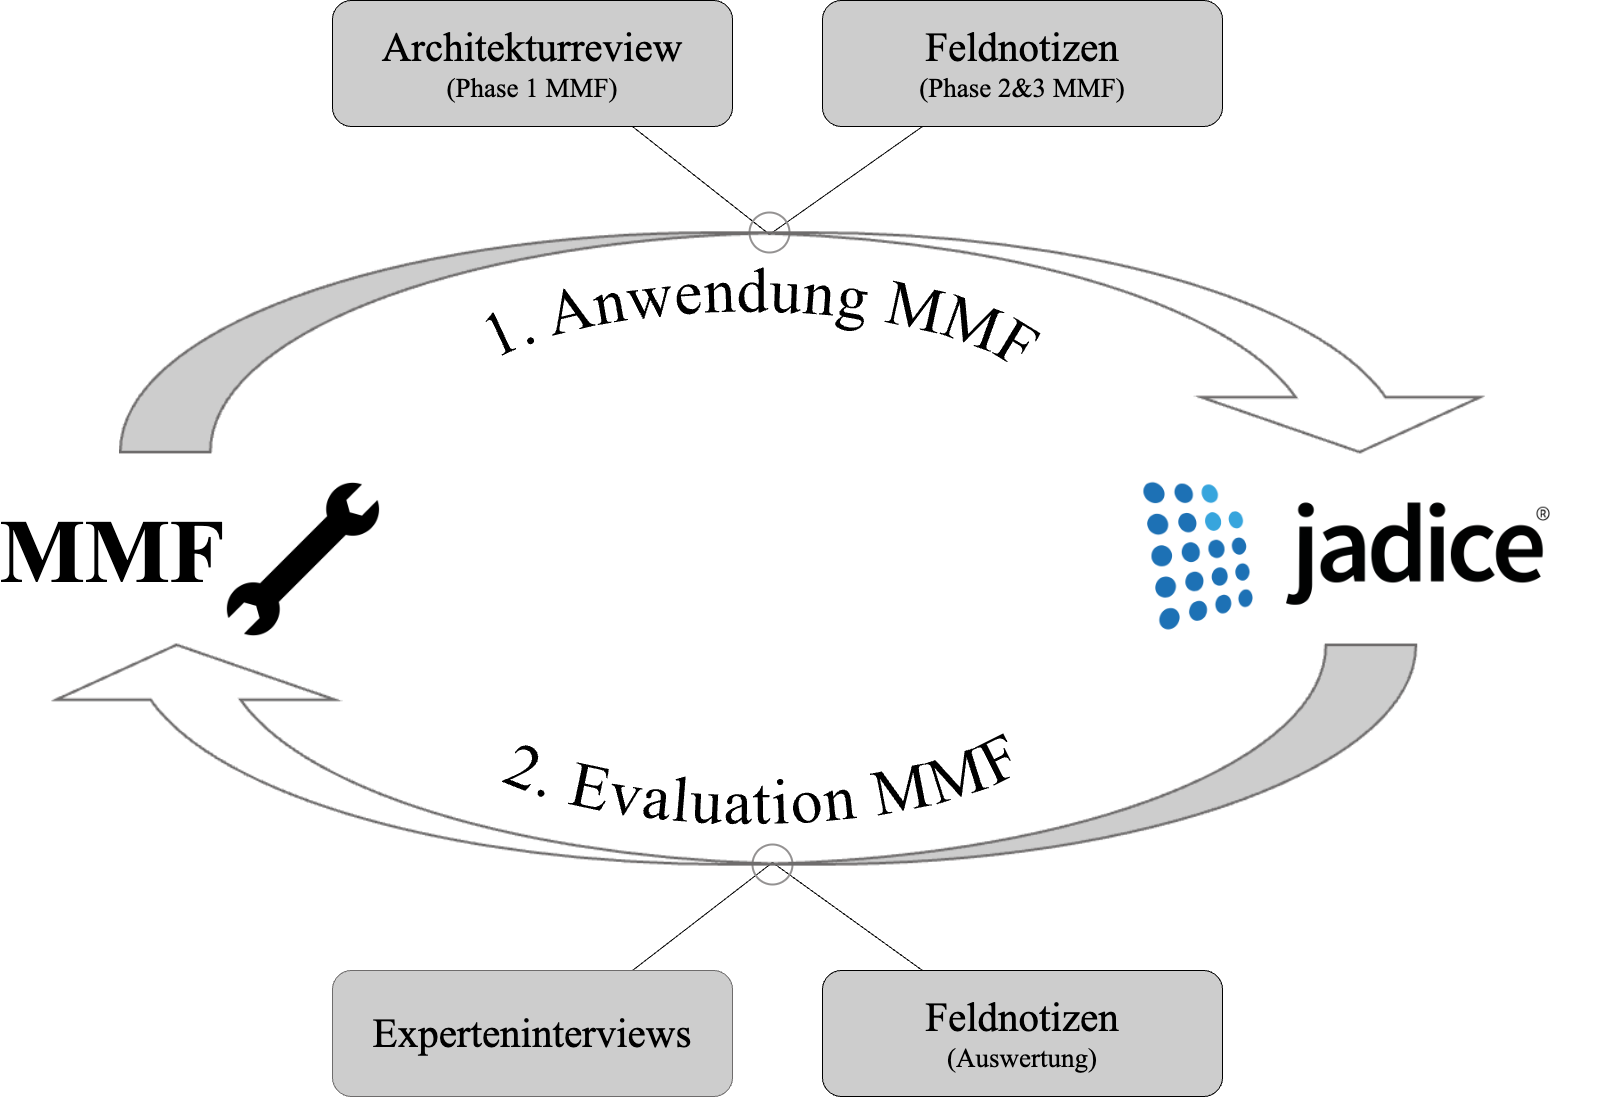
\includegraphics[width=0.7\textwidth]{methodology.drawio}
	\caption[Überblick über die Methodik dieser Fallstudie]{
		Überblick über die Methodik dieser Fallstudie.
	}
	\label{fig:methodology}
\end{figure}

\section{Anwendung des MMF}

Die Vorgehensweise beim Refactoring ist durch das Framework sehr genau vorgegeben.
Daher wird das Refactoring in dieser Thesis in die gleichen drei Phasen unterteilt wie in \cref{sec:mmf} beschrieben.
In der ersten Phase wird gemeinsam mit den Stakeholdern des Produkts ein Architekturreview nach \Citet{SVAHNBERG20071893} durchgeführt.
Diese Methode wird in \cref{sec:methodik-architekturreview} näher beschrieben.
Das wesentliche Ergebnis dieses Reviews sind die gewünschten \glspl{qa} des Systems.
Diese Attribute sind die Basis für Phase 2 und 3 und werden in den \gls{arh} eingegeben.
Dieser führt Berechnungen mit den \glspl{qa} durch und kann so eine Liste von Refactoring-Methoden vorschlagen, die nach ihrer Eignung für die \glspl{qa} sortiert sind.
Als weitere Eingabe für diese Suche dienen bestimmte Filter, die in \cref{sec:durchführung-phase2} näher erläutert werden.
Aus der resultierenden Liste von Migrationsmethoden werden die besten Vorschläge betrachtet und bewertet, bevor einer davon ausgewählt und in den folgenden Phasen verwendet wird.
Analog dazu wird in Phase 3a auf Basis der \glspl{qa} und Filter aus Phase 2 eine sortierte Liste von Patterns und Best Practices vorgeschlagen.
Das Vorgehen bei der Auswahl der Filter sowie die spätere Inspektion der Vorschläge des \gls{arh} werden in Form von strukturierten Feldnotizen protokolliert.
Deren genauere Funktion und Form wird in \cref{sec:structured-field-notes} näher erläutert.

\subsection{Architekturreview}
\label{sec:methodik-architekturreview}

Die Methodik eines Architekturreviews wird in dieser Thesis nach Vorschlag des \gls{mmf}/\gls{arh} dazu verwendet, Qualitätsanforderungen an das System, sogenannte \acrfullpl{qa}, zu sammeln.
Für Konformität mit dem Tool \gls{arh}, das als Ergebnis des Architekturreviews Szenarien benötigt, die \acrfullpl{qa} beschreiben, beschränkt sich die Auswahl möglicher Verfahren für die erste Phase auf szenarienbasierte Architekturreviews.
Das bedeutet, dass die gewünschten \glspl{qa} des Systems in Form von Szenarien erfasst und dokumentiert werden.
Ein Szenario beschreibt dabei eine Interaktion eines Stakeholders mit dem Produkt \cite{kazman_2000}.
Diese Konkretisierung von Qualitäten soll vor allem die Verständlichkeit fördern.
Dabei werden mit jedem Szenario zugehörige \glspl{qa} assoziiert, wodurch am Ende eine Abbildung aller \glspl{qa} auf ihre Priorität möglich ist.
Diese Abbildung ist das eigentliche Ergebnis, das der \gls{arh} als Eingabe für die weiteren Phasen benötigt.
Die Szenarien sind dabei lediglich ein Zwischenprodukt und sollen dabei helfen, eine genauere Vorstellung davon zu bekommen, welche spezifischen Situationen mit den \glspl{qa} verbunden sind.
Sie ermöglichen auch eine Bewertung der Wichtigkeit und technischen Schwierigkeit anhand konkreter Situationen, was bei abstrakten \glspl{qa} schwieriger wäre.

Folgend werden verschiedene akademische Methoden beschrieben und verglichen und anschließend die verwendete Methode als Abwandlung dieser Methoden erläutert.

\subsubsection{Vergleich verschiedener Methoden}
\label{sec:atam-saam-svahnberg}

Geläufige szenarienbasierte Verfahren sind die \gls{saam} nach \Citet{saam} und die \gls{atam} nach \Citet{kazman_2000}.
\gls{atam} ist der Nachfolger und eine Überarbeitung von \gls{saam}, weshalb folgend lediglich \gls{atam} näher betrachtet wird.
Die Autoren beschreiben mit \gls{atam} eine Methode, die aus insgesamt neun Schritten besteht.
Diese Schritte sollen mit den Stakeholdern des Produkts innerhalb von drei Arbeitstagen durchgeführt werden.
Da das Ausmaß dieser allerdings nicht angemessen für den Rahmen einer Thesis ist \cite{master-marvin-knodel}, würde für diese Arbeit höchstens eine stark abgewandelte Version dieser infrage kommen.
Stattdessen wurde sich in dieser Thesis für eine Modifikation des Architekturreviews nach \Citet{SVAHNBERG20071893} entschieden.
Es handelt sich dabei ebenfalls um eine szenarienbasierte Methode, die auf \gls{saam} und \gls{atam} basiert, jedoch spezieller für kleinere Anwendungsfälle entwickelt wurde.
Die Autoren erläutern die Verwendung dieser zur Evaluation von Studentenprojekten, die ein reales Softwareentwicklungsprojekt mit Industriekunden simulieren und einen Rahmen von 10-15 Teilnehmern und 20 Wochen Arbeitszeit vorsehen.

\subsubsection{Architekturreview nach \Citet{SVAHNBERG20071893}}

Das Architekturreview nach  \Citet{SVAHNBERG20071893} umfasst sechs Schritte (Übersicht in \cref{tab:svahnberg-plan}).
\begin{table}[!h]
  \centering
  \begin{tabular}{l l}
    \toprule
    \textbf{Aktivität} & \textbf{Zeit (in Minuten)} \\ \midrule
    1. Einleitung in das Projekt & 15 \\
    2. Identifikation von Qualitätsanforderungen & 20 \\
    3. Szenarienerhebung & 45 \\
    ~~~~Pause & 20 \\
    4. Architekturpräsentation & 20 \\
    5. Szenario- und Architekturanalyse & 90 \\
    6. Fazit & 15 \\
    \bottomrule
  \end{tabular}
  \caption[Zeitplan für ein Architekturreview nach \Citet{SVAHNBERG20071893}]{
    Zeitplan für ein Architekturreview nach \Citet{SVAHNBERG20071893}.
  }
  \label{tab:svahnberg-plan}
\end{table}

Diese sollen in einer etwa vierstündigen, mo\-de\-rierten Gruppendiskussion mit den wichtigsten Stakeholdern des Produkts durchgeführt werden.
Im ersten Schritt gibt der \gls{po} eine Einführung in das Projekt, in der Ziele für das Produkt sowie die Organisation geschildert werden.
Im zweiten Schritt wird in einer Brainstorming-Runde zusammen mit dem \gls{po}, End-Nutzern und Architekten die Identifikation von \glspl{qa} durchgeführt.
Hierfür dient die Liste der Qualitätskriterien gemäß ISO 9126~\cite{ISO-9126} als Vorlage für mögliche \glspl{qa}.
Im dritten Schritt ordnen \gls{po} und End-Nutzer die Liste der \glspl{qa} nach ihrer Wichtigkeit und fügen den drei wichtigsten jeweils zwei Szenarien hinzu.
Nach einer Pause präsentiert im vierten Schritt ein Softwarearchitekt die vorgeschlagene Architektur.
Anschließend werden im fünften Schritt die Szenarien sequenziell analysiert und bewertet, inwiefern sie durch die Architektur erfüllt werden und wo etwaige Probleme bestehen.
Im sechsten Schritt werden alle identifizierten Probleme und Aspekte, die mehr Aufmerksamkeit benötigen, final diskutiert und der gesamte Prozess zusammengefasst.

\subsubsection{Anpassung des Architekturreviews auf den \gls{arh}}

Ein volles Architekturreview, auf Deutsch auch mit Architekturbewertung zu übersetzen, ist generell bei der Verwendung des \gls{arh} und somit in dieser Thesis nicht das primäre Ziel.
Vielmehr entfällt das Hauptziel eines herkömmlichen Architekturreviews: die Bewertung.
Stattdessen wurde die in \cref{tab:architekturreview-plan} dargestellte Methodik zur Extraktion von Szenarien und \glspl{qa} entworfen.
\begin{table}[!h]
  \centering
  \begin{tabular}{m{4.4cm} m{7.6cm} p{1.3cm}}
    \toprule
    \textbf{Schritt nach \Citet{SVAHNBERG20071893}} & \textbf{Sub-Schritt} & \textbf{Zeit} \\ \midrule
    1. Einleitung in die Me\-tho\-dik & & 10 min\\ \hline
    \multirow{2}{=}[0cm]{2. Identifikation von Qualitätsanforderungen} & 1. Umfrage über wichtigste drei Sub-\glspl{qa} &  \multirow{3}{=}[0.2cm]{20 min}\\
    & 2. Diskussion über Priorisierung der Sub-\glspl{qa} & \\ \hline
    \multirow{3}{=}[-0.3cm]{3. Szenarienerhebung} & 1. Erstellen Szenarien zu wichtigsten Sub-\glspl{qa}& \multirow{3}{=}[-0.3cm]{60 min}\\
    & 2. Hinzufügen Wichtigkeit \& technische Schwie\-rig\-keit zu Szenarien  & \\
    & 3. Szenarien mit weiteren \glspl{qa} assoziieren  & \\ \hline
    5. Szenario- und Archi\-tek\-tur\-analyse & 1. Architekturbewertung anhand der Szenarien & 10 min \\
    \bottomrule
  \end{tabular}
  \caption[Zeitplan für das durchgeführte Architekturreview]{
    Zeitplan für das in Phase 1 dieser Thesis durchgeführte Architekturreview.
  }
  \label{tab:architekturreview-plan}
\end{table}


Wie in der Tabelle angemerkt, dienen als Vorlage für die Methodik die ersten Schritte des Ar\-chi\-tek\-turreviews nach \Citet{SVAHNBERG20071893}.
Außerdem werden auch einzelne Aspekte von \gls{atam} \cite{kazman_2000} verwendet.
Die einzelnen Schritte werden folgend näher beschrieben.

Im ersten Schritt ist die Einleitung in die Methodik geplant.
Dabei handelt es sich um eine Mo\-di\-fi\-ka\-ti\-on des nach \Citet{SVAHNBERG20071893} geplanten ersten Schritts, bei dem stattdessen eine Einleitung in das Projekt erfolgt.
Dieser stammt vermutlich aus dem Kontext der Studentenprojekte, bei denen mehrere Architekturreviews am selben Tag von den gleichen Personen durchgeführt werden und somit eine Einleitung in das Projekt nötig ist.
In den meisten Fällen in der Industrie, und so auch in diesem, ist dieser Schritt nicht notwendig, da die Teilnehmer der Besprechung, die Stakeholder, bereits mit dem Produkt vertraut sind.
Stattdessen wird (wie in \gls{atam} \cite{kazman_2000}) im ersten Schritt eine Einleitung in die verwendete Methodik gegeben, da diese dem Team noch unbekannt war.

Mit Schritt 2 beginnt das eigentliche Architekturreview.
Dabei werden die wichtigsten \glspl{qa} in zwei Sub-Schritten gesammelt:
Zunächst erfolgt eine Umfrage, bei der die Teilnehmer jeweils eine Einschätzung über die drei wichtigsten Sub-\glspl{qa} abgeben.
Anschließend wird in einer gemeinsamen Diskussion eine Priorisierung der Sub-\glspl{qa} finalisiert.
Als Basis-\glspl{qa} werden statt der ISO 9126~\cite{ISO-9126} nach \Citet{SVAHNBERG20071893} die von \Citet{master-daniel-koch} speziell für Microservices-Architekturen identifizierten \glspl{qa} verwendet.
Diese \glspl{qa} sind in \cref{fig:qas} dargestellt.
\begin{figure}[!h]
	\centering
	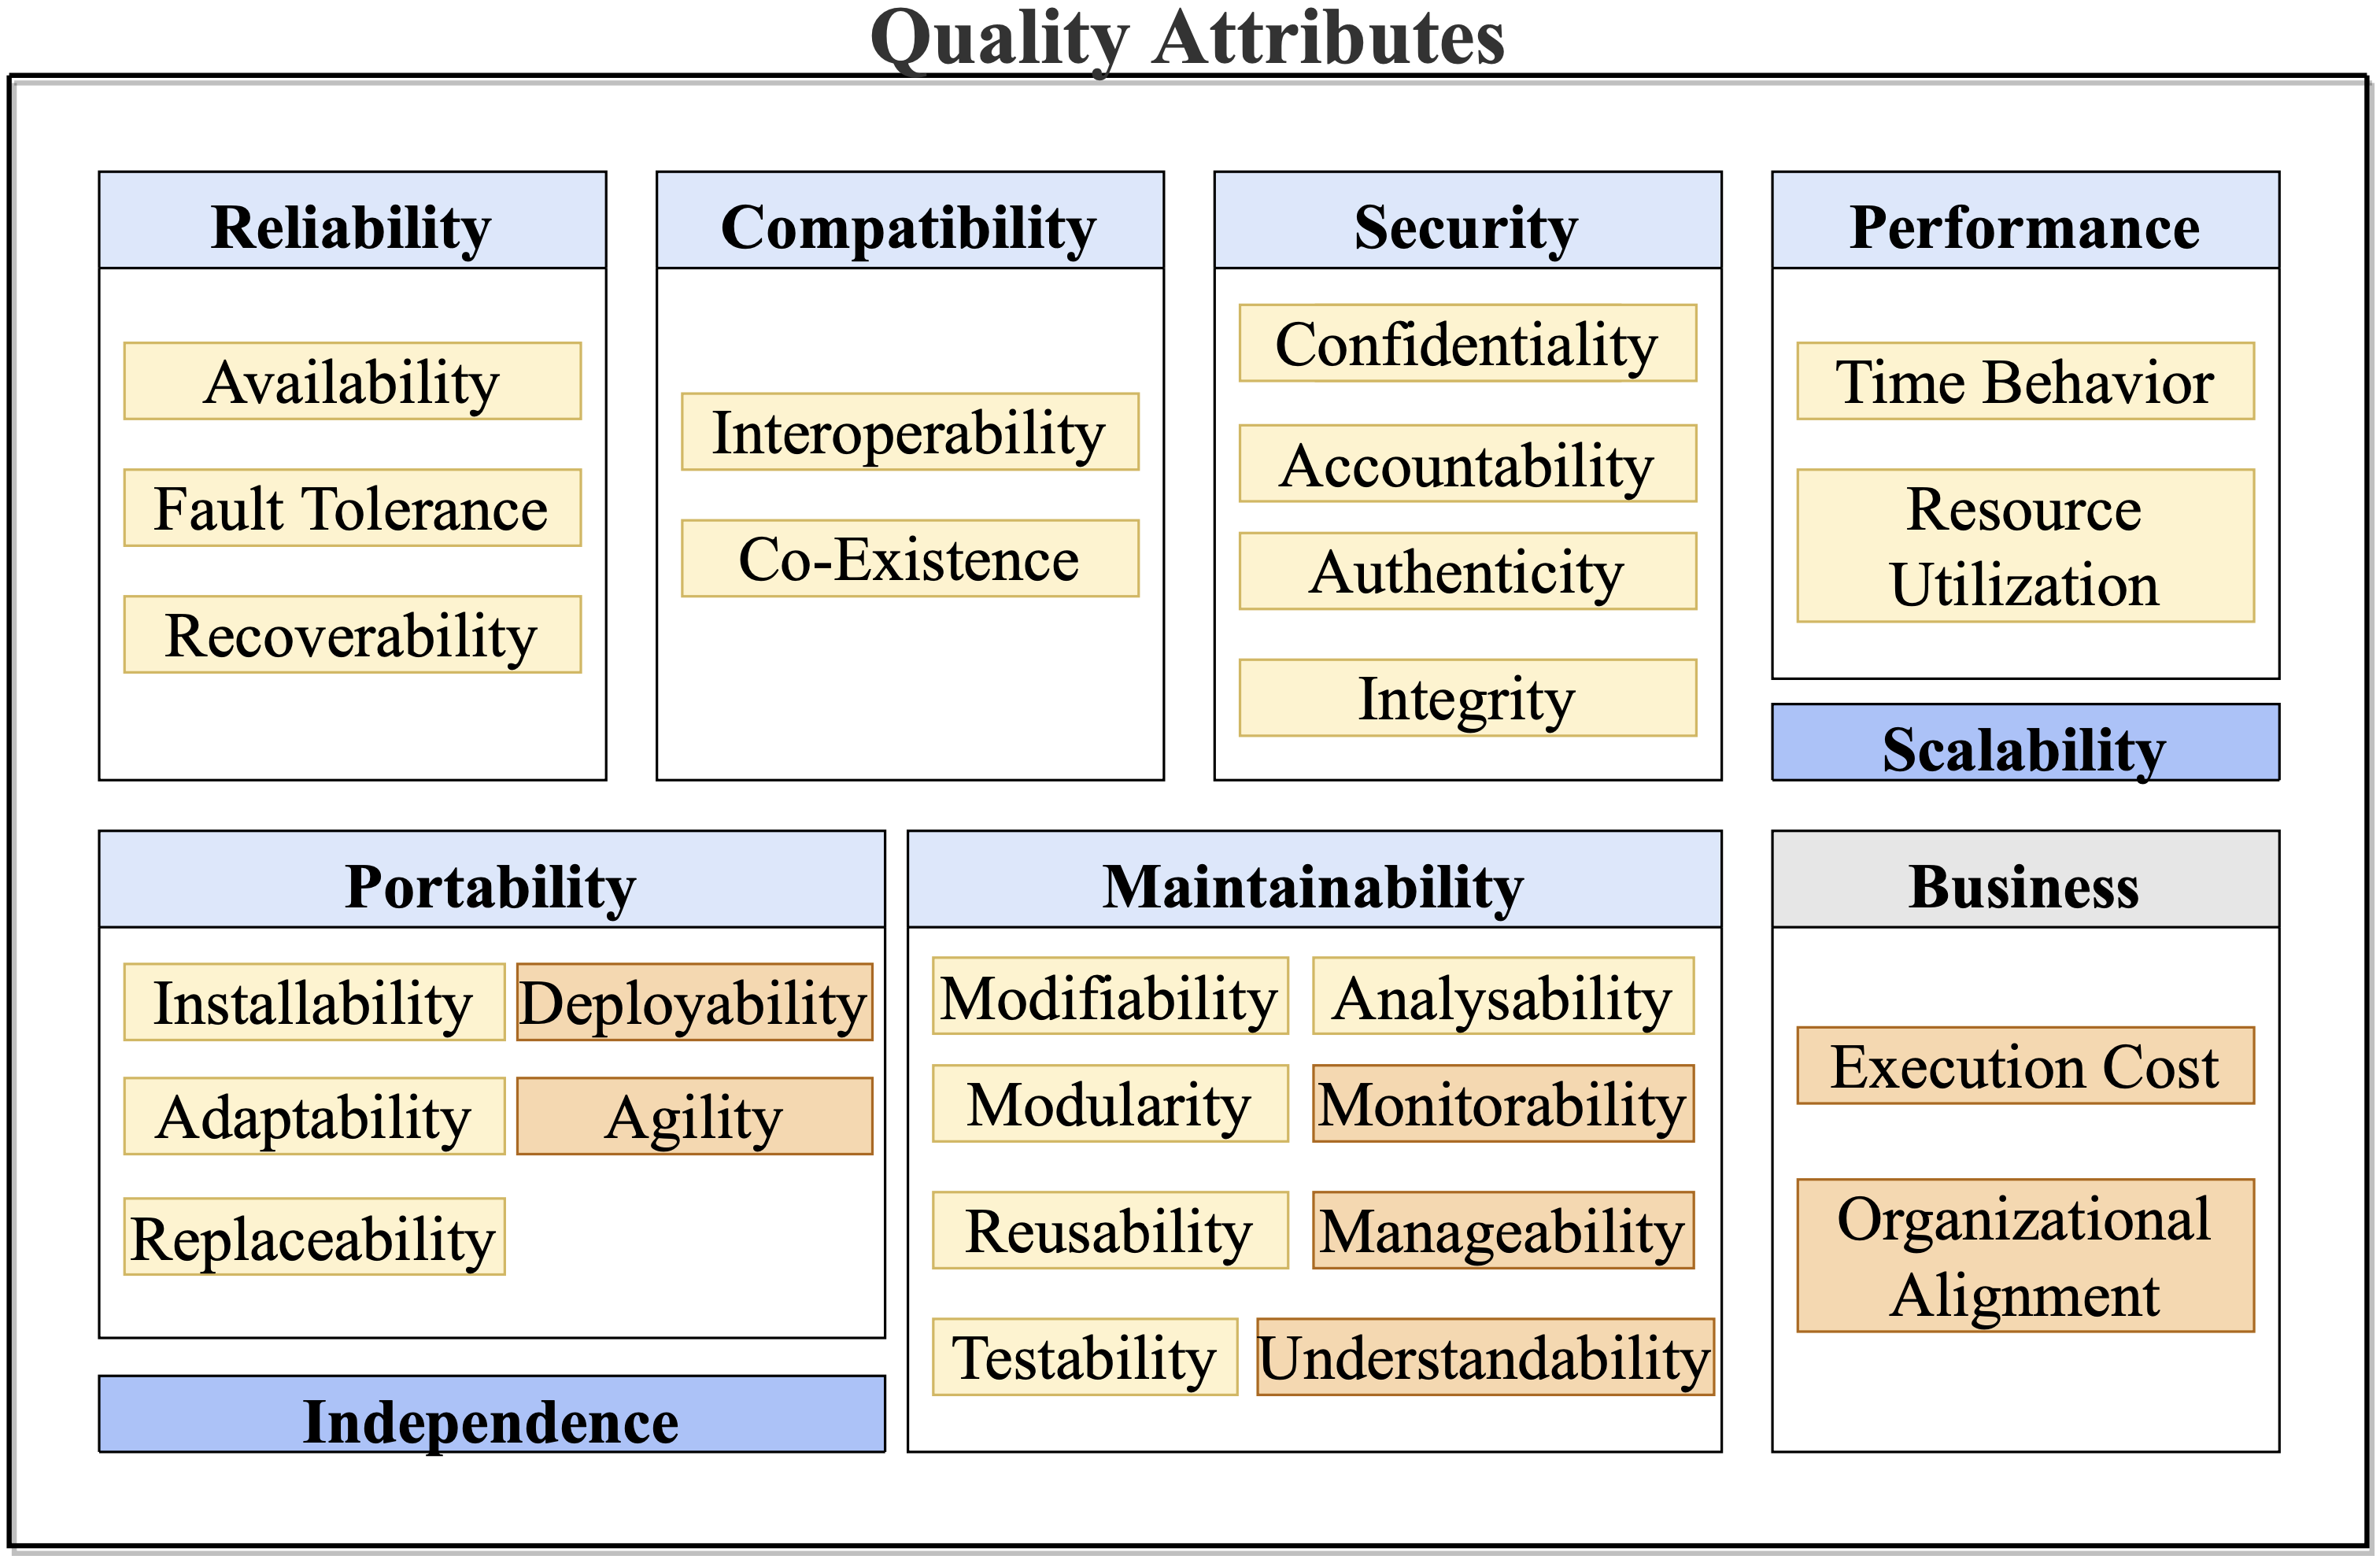
\includegraphics[width=0.7\textwidth]{qas}
	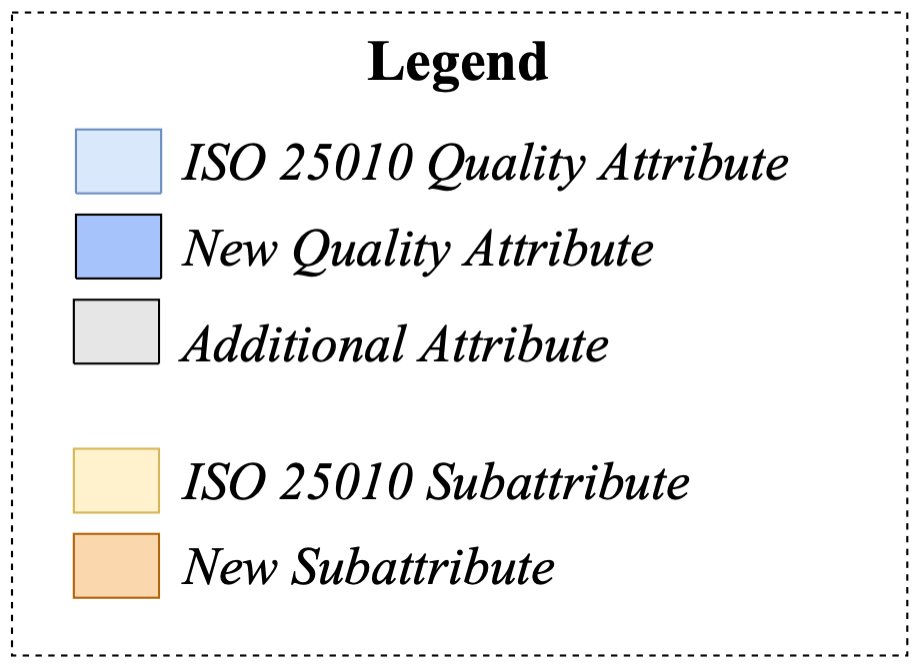
\includegraphics[width=0.3\textwidth]{qas-legend.drawio}
	\caption[Spezielle \acrlongpl{qa} für Microservices-Architekturen]{
		Spezielle \acrfullpl{qa} für Microservices-Architekturen nach \Citet{master-daniel-koch}.
	}
	\label{fig:qas}
\end{figure}
Es handelt sich hierbei größtenteils um die wichtigsten \glspl{qa} aus der ISO 25010 \cite{ISO-25010}, die durch einige spezifische \glspl{qa} für Microservices ergänzt wurden.
Aufgrund der Verwendung des \gls{arh} ist es sinnvoll, diese zu nutzen, da der \gls{arh} nur diese zulässt.

Die im zweiten Schritt erstellte Priorisierung der \glspl{qa} wird im dritten Schritt dann verwendet, um Szenarien zu erstellen.
Dieser ist in drei Sub-Schritte unterteilt:
Erst werden für die wichtigsten \glspl{qa} Szenarien erstellt.
Diese werden in Form eines Utility festgehalten (siehe \cref{fig:utility-tree}).
Dann wird inspiriert von \gls{atam} \cite{kazman_2000} jedes Szenario erneut betrachtet und eine Bewertung hinsichtlich der Wichtigkeit und technischen Schwierigkeit vorgenommen.
Diese erfolgt auf einer Skala von A bis C, wobei A für die höchste Wichtigkeit und höchste technische Schwierigkeit steht.
Abschließend wird jedes Szenario ein drittes Mal betrachtet und die Assoziation mit anderen \glspl{qa} diskutiert und festgehalten.
Bei diesem Schritt stammt nur der erste Teil aus der Methodik von \Citet{SVAHNBERG20071893} und die anderen beiden Schritte stammen aus dem \gls{arh}.
Dass bei der Vorlage von \Citet{SVAHNBERG20071893} keine vergleichbare Bewertung der Szenarien und Assoziation der Szenarien mit weiteren \glspl{qa} beschrieben ist, liegt vermutlich am Kontext des Architekturreviews.
Im Kontext der qualitativen Bewertung durch Menschen sind diese nicht explizit notwendig.
Im Vergleich dazu können bei der automatisierten Auswertung durch ein Werkzeug wie den \gls{arh} die Szenarien nicht selbstständig eingeschätzt werden.
Außerdem stammt die Visualisierung durch einen Utility Tree aus \gls{atam} \cite{kazman_2000}.
Ein solcher soll dabei helfen, Qualitätsziele zu konkretisieren und zu priorisieren \cite{kazman_2000}.
Dabei werden nach einem semantisch unbedeutenden Wurzelknoten von links nach rechts die \glspl{qa} in Sub-\glspl{qa} verfeinert, worauf dann auf dritter Ebene Szenarien folgen.
Wie in \cref{fig:utility-tree} zu sehen ist, enthält die in dieser Thesis verwendete Notation des Utility Trees auch die Einschätzung der Szenarien in Wichtigkeit und technische Schwierigkeit.
\begin{figure}[!h]
	\centering
	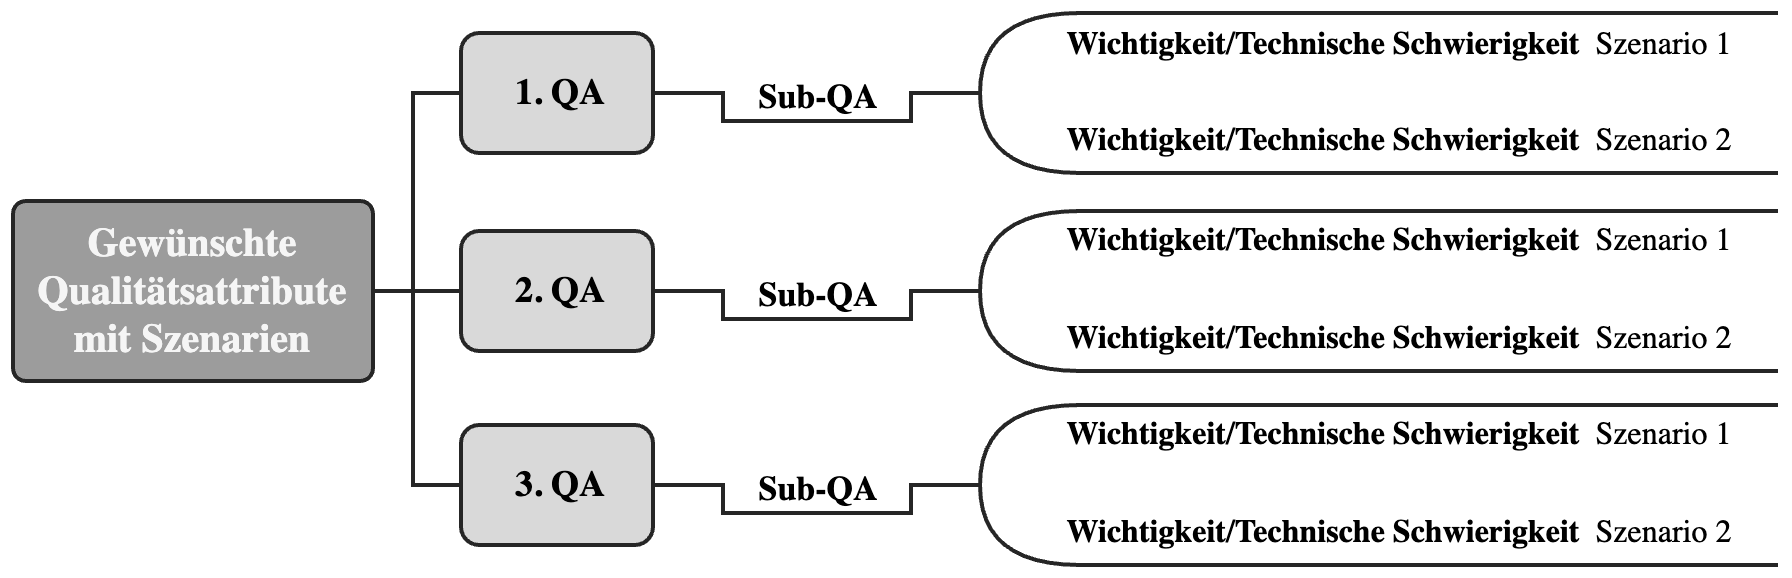
\includegraphics[width=\textwidth]{utility-tree.drawio}
	\caption[Utility Tree nach \acrshort{atam}]{
		Utility Tree nach \gls{atam} \cite{kazman_2000}, der auf die Verwendung mit dem \gls{arh} angepasst ist.
	}
	\label{fig:utility-tree}
\end{figure}


Im letzten Schritt erfolgt eine Bewertung, bei der jedem Szenario zugeordnet wird, ob eine \gls{msa} dafür vorteilhaft ist.
Diese Bewertung kann als Teil des fünften Schritts nach \Citet{SVAHNBERG20071893} gesehen werden.
Abgesehen davon wird allerdings der Teil der Bewertung der Architektur unter den Szenarien im Architekturreview komplett ausgelassen und der Rest der Schritte 4, 5 und 6 nach \Citet{SVAHNBERG20071893} nicht durchgeführt.
Während bei allen genannten szenarienbasierten Verfahren die Szenarien und \glspl{qa} lediglich ein Zwischenprodukt und Mittel zur Bewertung der Systemarchitektur sind, stellen sie bei dem im Rahmen dieser Thesis durchgeführten Architekturreview das gewünschte Endprodukt dar.

Die vorgestellte Methodik kann als neue Methodik zur Extraktion von Szenarien und \glspl{qa} betrachtet werden und könnte in Zukunft als Vorlage für die Anwendung mit dem \gls{arh} verwendet werden.
Trotz des Fehlens des Bewertungsschritts der Methodik wird sie folgend zur Vereinfachung als Architekturreview bezeichnet.

\subsection{Strukturierte Feldnotizen}
\label{sec:structured-field-notes}
Während Phase 1 mit der Methodik einer Fokusgruppe durchgeführt wird, findet die Bearbeitung in den fol\-gen\-den Phasen größtenteils in Einzelarbeit statt.
Um dabei strukturiert zu protokollieren, welche Aktivitäten im Rahmen dieser Phasen durchgeführt werden, werden systematisch durch\-ge\-führte Aktivitäten mit gemachten Erfahrungen und Herausforderungen dokumentiert. %und am Ende aus\-ge\-wer\-tet.
Dazu werden wie in der ähnlichen Arbeit von \Citet{master-marvin-knodel} strukturierte Feldnotizen nach \Citet{seaman2008qualitative} verwendet.

Jede Feldnotiz wurde zeitnah nach Beobachtung in einer zugehörigen Datei mit dem Na\-mens\-sche\-ma F\emph{Nummer}\_P\emph{Phase\gls{mmf}}\_\emph{Datum}\_\emph{Name}.tex erstellt.
Dabei wurden dementsprechend Nummer der Feldnotiz, Phase des \gls{mmf}, Datum (im Format \emph{MM\_DD\_JJJJ}) und Name der Feldnotiz im Dateinamen festgehalten.
\cref{feldnotiz:1} hat beispielsweise den Namen \emph{F01\_P2\_11\_20\_2023\_FilterAuswahl.tex}.
\cref{tab:field-notes} gibt einen Überblick über die Eintrags-Felder und welchem Feld nach \Citet{seaman2008qualitative} sie entsprechen.

\begin{table}[!h]
  \centering
  \begin{tabular}{l m{7cm}}
    \toprule
    \textbf{Eintrag} & \textbf{Eintrag nach \Citet{seaman2008qualitative}} \\ \midrule
    Feldnotiz Nr. & -  \\ \hline
	Datum, Uhrzeit & Zeit  \\ \hline
	Ort	 & Ort \\ \hline
	Beteiligte Personen	 & Teilnehmer der Beobachtung \\ \hline
	Phase \& Schritt des \gls{mmf} & Verfolgte Ziele  \\ \hline
	Aktionen und Entscheidungen & Stattgefundene Handlungen und Diskussionen\\ \hline
	Kommentare & Kommentare \\ \hline
	Was lief gut & Diskussion \\ \hline
	Probleme & Diskussion \\ \hline
	Empfindungen &Ton und Stimmung der Interaktionen \\
    \bottomrule
  \end{tabular}
  \caption[Aufbau der strukturierten Feldnotizen nach \Citet{seaman2008qualitative}]{
  	Aufbau der strukturierten Feldnotizen nach \Citet{seaman2008qualitative}.
  }
  \label{tab:field-notes}
\end{table}


\section{Evaluation des MMF}

Das Forschungsziel dieser Arbeit ist die Evaluation des \gls{mmf} und des \gls{arh}.
Nach dem Refactoring von \jf mit dem Framework wird evaluiert, als wie hilfreich sich dieses bei der Optimierung einer bereits vorhandenen \gls{msa} herausgestellt hat.
Dafür werden Experteninterviews durchgeführt sowie die im Verlauf der Anwendung erstellten Feldnotizen ausgewertet.

\subsection{Experteninterviews}
\label{sec:methodik-interviews}
Im Rahmen dieser Arbeit werden Experteninterviews durchgeführt, um die Nützlichkeit des \gls{mmf} und \gls{arh} bei der Migration zu Microservices im Spezialfall \jf zu evaluieren.
Interviews im Software Engineering allgemein werden oft genutzt, um Softwareprozesse zu bewerten \cite{seaman2008qualitative}.

\subsubsection{Aufbau}
Es gibt verschiedene Arten von Interviews sowie viele verschiedene Vorgehensweisen bei der Planung, Durchführung und Auswertung der Interviews.
In den nächsten Abschnitten wird beschrieben und begründet, welche Art und welche Vorgehensweisen verwendet werden.

\paragraph{Art:} Ein wichtiges Unterscheidungsmerkmal bei Interviews ist die Offenheit der Fragen.
\Citet{seaman2008qualitative} beschreibt zwei Ausprägungen: strukturierte und unstrukturierte Interviews.
Während struk\-tu\-rier\-te Interviews klare Antworten auf spezifische Fragen erwarten, haben unstrukturierte Interviews den Vorteil, dass auch unvorhergesehene Informationen zu den Antworten auf offene Fragen gehören können.
Um die Vorteile beider Varianten zu kombinieren, werden in dieser Arbeit semi-strukturierten Interviews \cite{seaman2008qualitative} verwendet.
Dabei werden spezifische Fragen gestellt, aber auch offene Fragen mit eingebunden, um die Flexibilität der potentiellen Ergebnisse zu erhöhen.

\paragraph{Experten:} Wie aus dem Namen hervorgeht, ist die Auswahl der Experten eine wichtige Entscheidung bei der Planung von Experteninterviews.
Die für die Interviews relevante Expertise ist \glqq Betriebswissen\grqq{} \cite{Meuser2009}.
Als Experten wurden Mitarbeiter mit guter Kenntnis des Produkts \jf ausgewählt, da die Fragen einen besonderen Bezug zur Nützlichkeit des Frameworks für das Produkt haben.
\Citet{Runeson2009} empfehlen, aufgrund der qualitativen Natur von Fallstudien, möglichst verschiedene Teilnehmer auszuwählen, anstatt nach Ähnlichkeiten zu suchen.
Aus diesem Grund wurde bei der Wahl der Mitarbeiter nach ihrer Rolle in der Produktentwicklung von \jf differenziert.
Für die abstrakteste Perspektive auf das Produkt wurde der \acrlong{po} (nach Definition des SCRUM von \Citet{SCRUM}) ausgewählt.
Für die technische Perspektive wurde der \gls{se} hinzugezogen.
Als weitere Meinung einer Person, die zwischen den beiden genannten Rollen liegt, wurde der \gls{sa} herangezogen.

\paragraph{Protokollierung:} Zwei geläufige Optionen für die Aufnahme eines Interviews sind die Pro\-to\-kol\-lie\-rung während des Interviews, entweder durch den Interviewer oder einen separaten Protokollant \cite{seaman2008qualitative,Runeson2009}.
Der Interviewer selbst ist besonders im Fall von Unerfahrenheit keine gute Wahl, da es kompliziert sein kann, zwei Aufgaben gleichzeitig zu bewältigen und die Leitung des Interviews somit leiden kann.
Die Lösung durch einen Protokollanten ist auch nicht optimal, da ein solcher nicht immer zur Verfügung steht.
Außerdem kann es zu Interpretationsunterschieden kommen, welche Informationen relevant sind.
Deswegen wird, wie von \Citet{seaman2008qualitative} sowie \Citet{Runeson2009} empfohlen, eine Aufzeichnung durch Audioaufnahme verwendet.

\paragraph{Leitfaden:} Eine weitere wichtige Vorbereitung für ein gut geplantes Interview ist die Erstellung eines Leitfadens \cite{seaman2008qualitative,hove-anda-2005}, welcher den Plan des Vorgehens enthält.
Dieser muss nicht so strikt gegliedert sein wie ein Fragebogen, sondern soll neben den Fragen Notizen für den Interviewer enthalten, die bei der Leitung des Interviews helfen.
Der für diese Interviews konzipierte Leitfaden ist in \cref{chap:expert-interviews-leitfaden} zu finden.
Er besteht aus hauptsächlich drei Teilen.
Im ersten Abschnitt werden Verständnisfragen gestellt.
Diese sollen absichern, dass die Informationen aus dem Informationsbogen ausreichend verstanden wurden, um die folgenden Fragen sinnvoll beantworten zu können.
Im zweiten Teil werden allgemeine inhaltliche Fragen zur Evaluation des \gls{mmf} gestellt, ohne Bezug zur Anwendung in dieser Thesis.
Mithilfe mehrerer Fragen sollen mögliche alternative Funktionsweisen, die Phasen des Frameworks und potenzielle Probleme dessen evaluiert werden.
Der letzte Teil dient der Bewertung der spezifischen Anwendung des Frameworks in dieser Thesis.
Dazu werden zunächst Fragen zu den mit dem \gls{arh} ermittelten Migrationsverfahren gestellt.
Da ein gutes Verständnis der Verfahren dafür nötig ist, werden die Fragen weiter spezifiziert, falls der Kandidat bei offenen Fragen in falsche Richtungen abschweift oder keine Antwort findet.
Außerdem wird für Bezug zur \hyperref[forschungsfrage:1]{Forschungsfrage} die Auswirkung der Verfahren auf die Granularität des Systems befragt.
Anschließend werden die mit \gls{arh} erhaltenen \bpp bewertet.
Auch hier werden zunächst offene Fragen gestellt und am Ende eine Frage mit Bezug zu den Qualitätsaspekten aus der \hyperref[forschungsfrage:1]{Forschungsfrage} gestellt.
Zum Abschluss werden dem Interviewten noch zwei Fragen zur Gesamtbewertung der Anwendung des Frameworks vorgelegt.
Dabei soll er seine Einzelbewertungen der letzten Schritte zusammenfassen und ein Fazit ziehen.

\paragraph{Vorbereitungsmaterial:}
Die Einleitung eines Interviews sollte nur einen kleinen Teil ausmachen, da Zeit in Interviews wertvoll und oft knapp bemessen ist \cite{Runeson2009,hove-anda-2005,seaman2008qualitative}.
Aus diesem Grund wurden für die Interviews eine Präambel und ein Informationsbogen erstellt, welche die Teilnehmer im Voraus erhalten haben.
%Diese sind in \cref{chap:expert-interviews-preamble,chap:expert-interviews-infobogen} zu finden.
Diese sind in den Anhängen \hyperref[chap:expert-interviews-preamble]{B} und \hyperref[chap:expert-interviews-infobogen]{C} zu finden.
Die Prä\-am\-bel fasst die generellen Richtlinien für die Experteninterviews zusammen.
Dabei diente die Präambel von Bogner et al.\footnote{\url{https://github.com/xJREB/research-microservices-interviews/blob/master/interview-preamble.md}} als Vorlage.
Da der thematische Kontext des Interviews durch die Voraussetzung des Verständnisses von zwei Migrationsmethoden relativ komplex ist, wurde außerdem ein Informationsbogen erstellt, der bei der thematischen Einarbeitung helfen soll.
Darin werden alle wichtigen Konzepte erklärt, die in den Interviews behandelt werden.
Der Bogen enthält einen generellen Überblick über  \gls{mmf}/\gls{arh} sowie die Funktionsweisen der zwei diskutierten Migrationsverfahren.
Es wird jedoch nicht erwartet, dass die Teilnehmer alle Inhalte im Voraus vollständig verstehen, da (wie im Leitfaden beschrieben) anfangs eine Runde zur Klärung der Verständnisfragen stattfindet.

\subsubsection{Analyse der Daten}

Die Analyse qualitativer Daten ist oft ein Prozess der parallel zu der Datensammlung stattfindet \cite{Runeson2009}.
Es ist wichtig, einen gut strukturierten und systematischen Plan für die Datenanalyse zu haben, da die Erkenntnisse in der Analyse die Sammlung der nächsten Daten beeinflussen können.
Wie \Citet{seaman2008qualitative} empfiehlt, wurde die Datenanalyse deswegen im Voraus geplant.
Obwohl es empfehlenswert ist, die Auswertung durch mehrere Forschende durchzuführen, um Voreingenommenheit zu reduzieren \cite{Runeson2009}, wird sie in dieser Arbeit aufgrund mangelnder Ressourcen nur vom Autor durchgeführt.

Die Rohdaten liegen in Form von drei Audioaufnahmen vor, die jeweils etwa eine Stunde lang sind.
Die Audioaufnahmen werden mithilfe der von \Citet{Mayring2019} vorgestellten Techniken  \emph{Zusammenfassen} und \emph{Explikation} getrennt transkribiert (siehe \cref{fig:datenanalyse}).
Die Ergebnisse dieser Transkription werden auf zwei verschiedene Arten in diese Thesis übernommen.
Zum einen wird eine \emph{Strukturierung} nach \Citet{Mayring2019} durchgeführt.
Dabei werden für jede gestellte Frage die Antwort kategorisiert.
Das dafür entworfene \glqq ordinal geordnete Kategoriensystem\grqq{} nach \Citet{Mayring2019} ist in \cref{fig:kodierleitfaden} zu sehen.
Auf der anderen Seite werden die Transkripte sowie die Kodierungen in textueller Form aggregiert.
Eine Übersicht über die dadurch entstandenen aggregierten Zusammenfassungen ist in \cref{tab:expert-interviews-analysis} gegeben.

%Diese enthalten Sammlungen von langen Texten, welche folgend auf einen geringeren Umfang gekürzt werden, ohne dabei relevante Informationen zu verlieren.
%Dabei werden die Techniken \emph{Zusammenfassen}, \emph{Explikation} und \emph{Strukturierung} nach \Citet{Mayring2019} verwendet.
%Das Ergebnis daraus ist jeweils eine textuelle Zusammenfassung der aggregierten Ergebnisse pro Fragenabschnitt:
%\begin{itemize}
%	\item Evaluation des \gls{mmf}/\gls{arh} allgemein
%	\item Evaluation der ausgewählten Migrationsmethoden für \jf
%	\item Evaluation der \bpp für \jf
%	\item Evaluation der Anwendung des \gls{mmf}/\gls{arh} auf \jf insgesamt
%\end{itemize}
\begin{figure}[!ht]
	\centering
	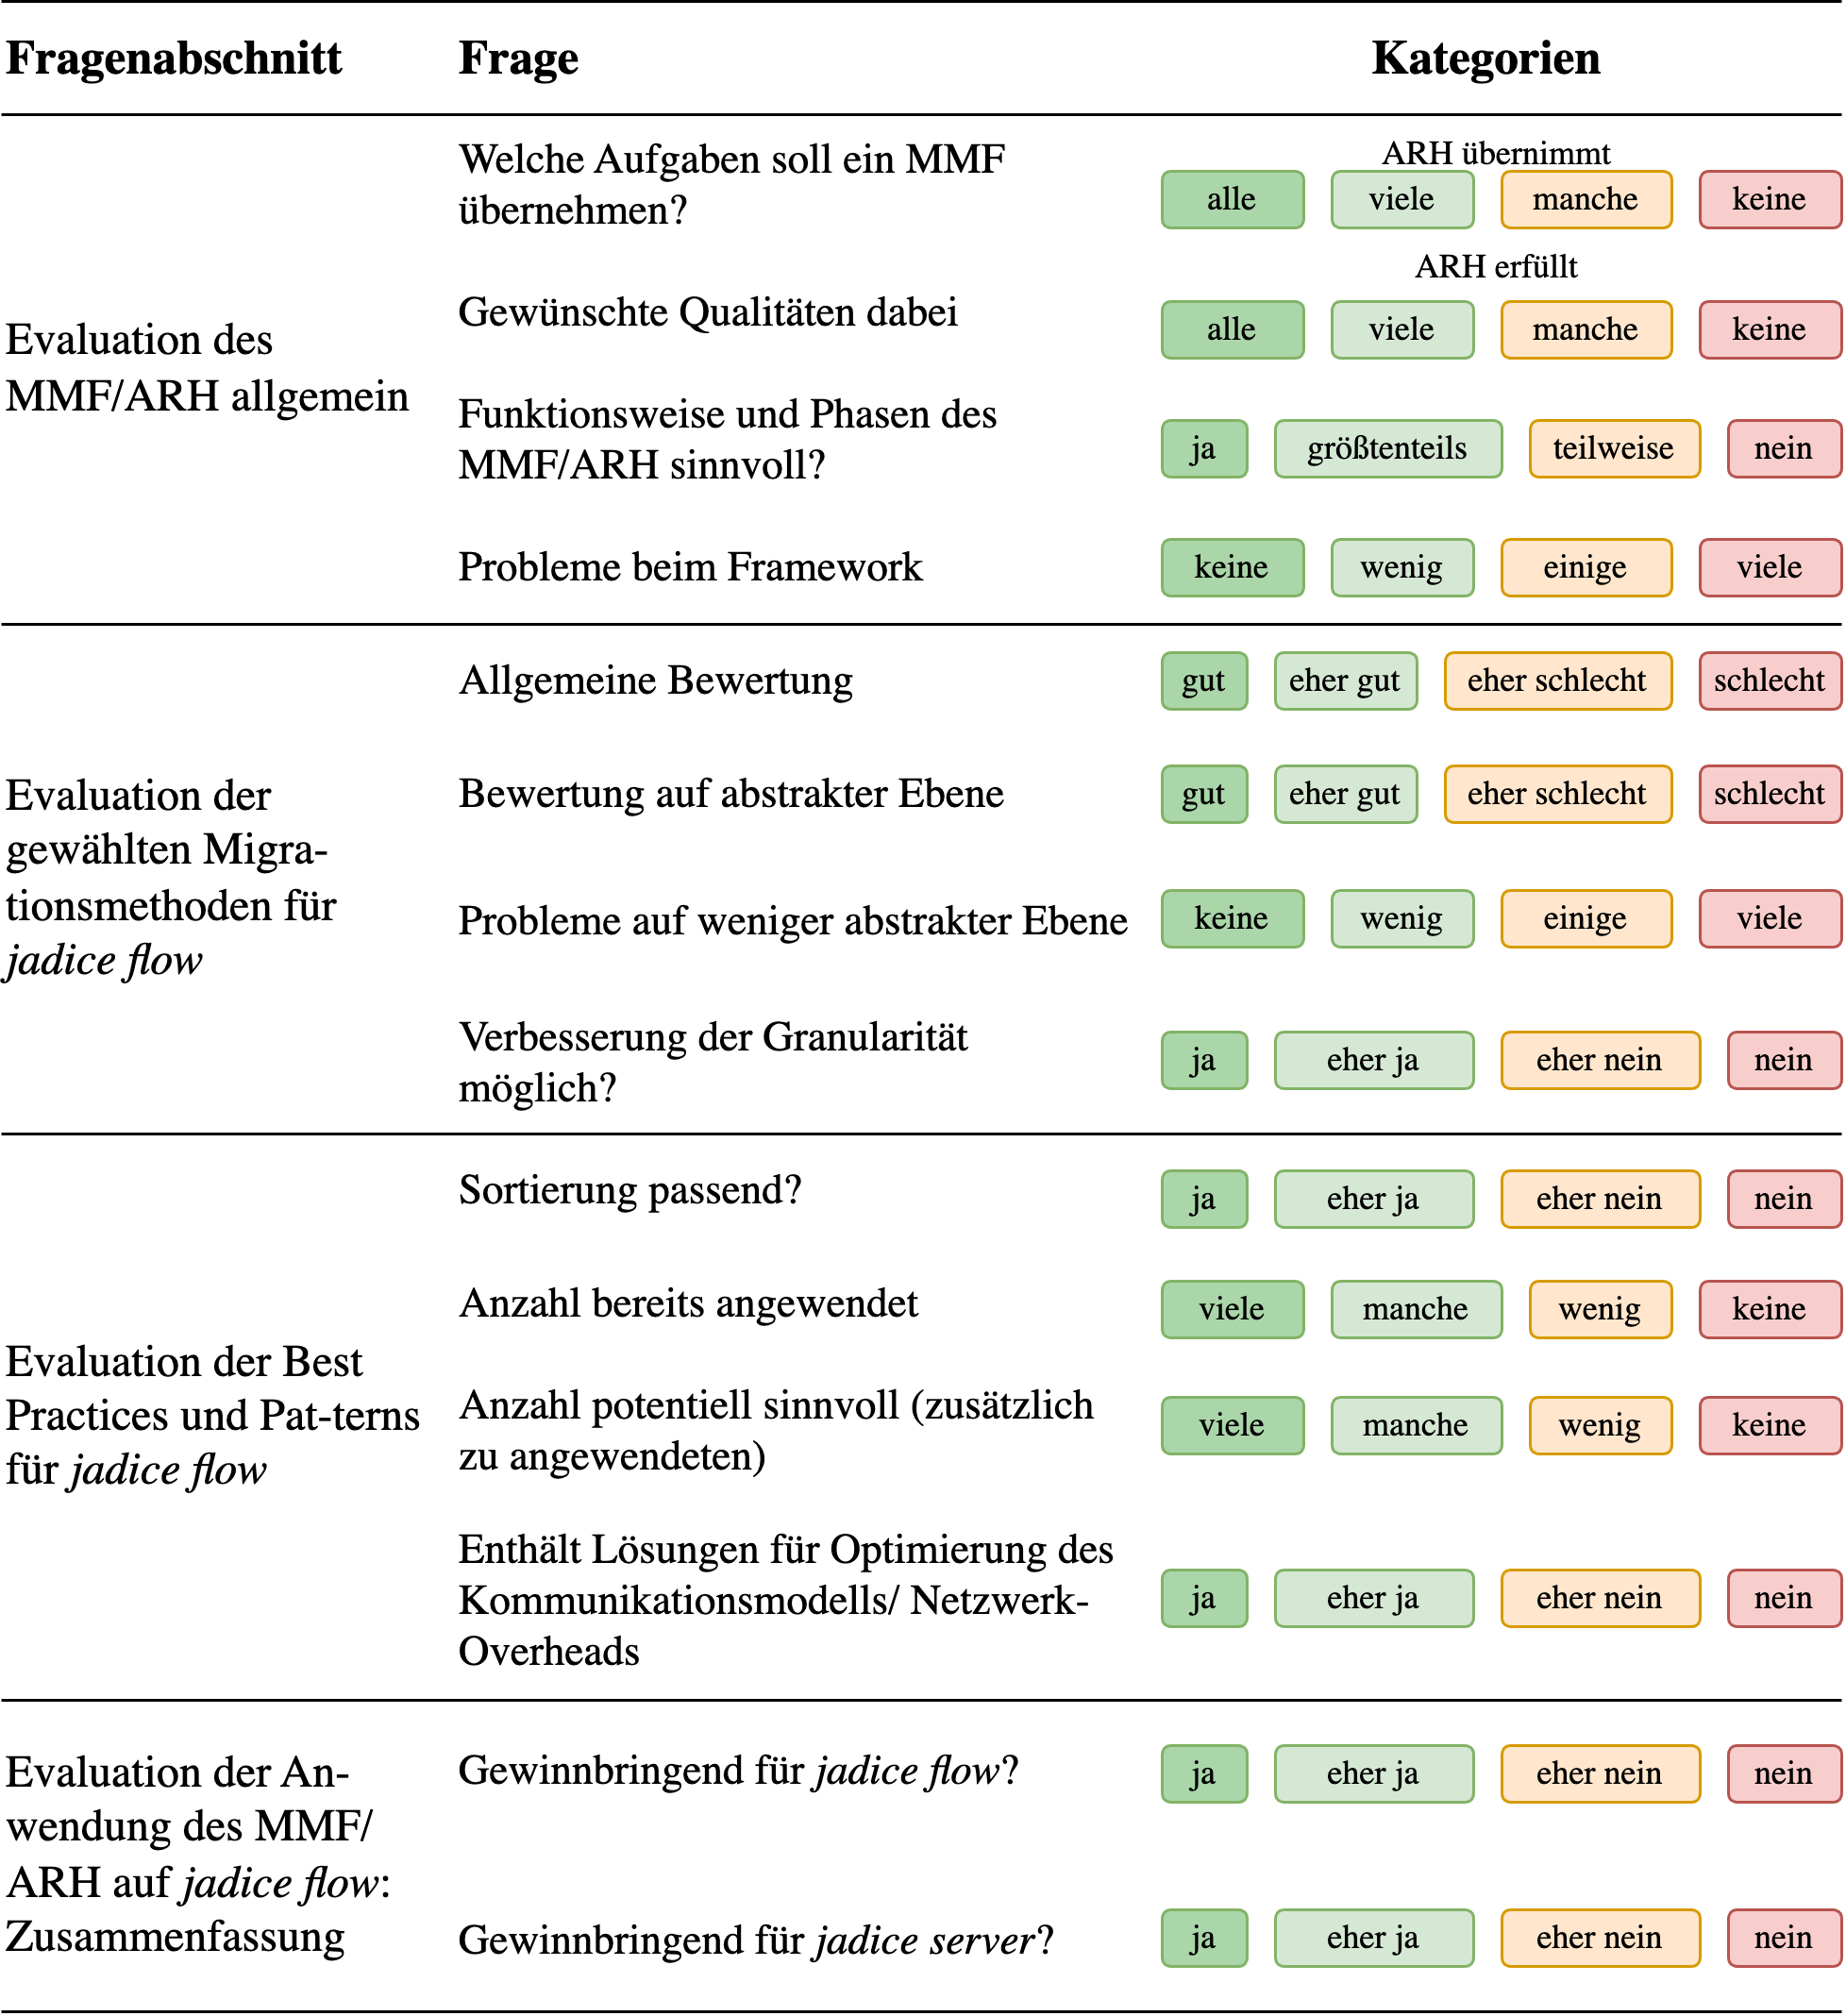
\includegraphics[width=\textwidth]{kodierleitfaden.drawio}
	\caption[Kodierleitfaden Auswertung Experteninterviews]{
		Kodierleitfaden für die Auswertung der Experteninterviews.
	}
	\label{fig:kodierleitfaden}
\end{figure}

\begin{figure}[!h]
	\centering
	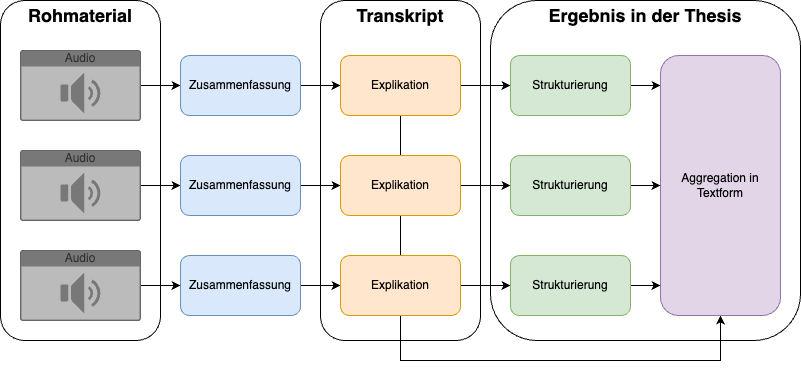
\includegraphics[width=0.8\textwidth]{Datenanalyse.drawio}
	\caption[Vorgehen Datenanalyse Experteninterviews]{
		Vorgehen bei der Datenanalyse der Experteninterviews.
	}
	\label{fig:datenanalyse}
\end{figure}


\begin{table}[!ht]
  \centering
  \begin{tabular}{m{5cm} m{6cm} l}
    \toprule
    \textbf{Kategorie} & \textbf{Fragenabschnitt} & \textbf{Abschnitt} \\ \midrule
    Evaluation des \gls{mmf}/\gls{arh} all\-ge\-mein & & \cref{sec:evaluation-mmf-allgemein} \\ \hline
%    \multirow{3}{=}[-0.6cm]{Evaluation der Anwendung des \gls{mmf}/\gls{arh} auf \jf} 
    & Evaluation der ausgewählten Mi\-gra\-ti\-ons\-me\-tho\-den für \jf & \cref{sec:evaluation-mmf-anwendung-methoden} \\
    Evaluation der Anwendung des \gls{mmf}/\gls{arh} auf \jf & Evaluation der \bpp für \jf & \cref{sec:evaluation-mmf-anwendung-bp-patterns} \\
     & Evaluation der Anwendung des \gls{mmf}/ \gls{arh} auf \jf insgesamt & \cref{sec:evaluation-mmf-anwendung-insgesamt} \\
    \bottomrule
  \end{tabular}
  \caption[Abschnitte der Auswertung der Experteninterviews]{
    Abschnitte der Auswertung der Experteninterviews
  }
  \label{tab:expert-interviews-analysis}
\end{table}




\subsection{Strukturierte Feldnotizen}
\label{sec:methodik-auswertung-feldnotizen}

Nachdem alle Feldnotizen erstellt sind, werden diese qualitativ ausgewertet.
Auch hier wird die Strukturierung nach \Citet{Mayring2019} verwendet.
Dafür wurde eine Kodierung erstellt, welche in \cref{tab:methodik-feldnitzen-kodierung} zu sehen ist.
An vielen Stellen wurde diese aus der ähnlichen Arbeit von \Citet{master-marvin-knodel} inspiriert.

\begin{table}[!h]
  \centering
  \begin{tabular}{l l m{7cm}}
    \toprule
    \textbf{Kodierung} & \textbf{Subkodierungen} & \textbf{Bedeutung} \\ \midrule
    Gut gelaufen            &              & Feldnotiz hat Eintrag bei \glqq Gut gelaufen\grqq{} \\ \hline
    Schlecht Gelaufen       &              & Feldnotiz hat Eintrag bei \glqq Schlecht gelaufen\grqq{} \\ \hline
    Mehr gut gelaufen       &              & Nach subjektiver Bewertung des Autors bei Betrachtung der Einträge in \glqq Gut gelaufen\grqq{} und \glqq Schlecht gelaufen\grqq{} ist mehr gut gelaufen \\ \hline
    Mehr schlecht gelaufen  &              & Nach subjektiver Bewertung des Autors bei Betrachtung der Einträge in \glqq Gut gelaufen\grqq{} und \glqq Schlecht gelaufen\grqq{} ist mehr schlecht ge\-laufen \\ \hline
    Gutes Gefühl            &              & Eintrag eines guten Gefühls in \glqq Em\-pfin\-dun\-gen\grqq{} \\ \hline
    \multirow{2}{*}[0cm]{Schlechtes Gefühl} & Unsicherheit & Eintrag eines Gefühls von Unsicherheit in \glqq Em\-pfindungen\grqq{} \\
                            & Frustration  & Eintrag eines Gefühls von Frustration in \glqq Em\-pfindungen\grqq{} \\ \hline
    Verbesserungsvorschlag  &              & In der Feldnotiz ist direkt oder in\-di\-rekt in einem beliebigen Feld ein Ver\-bes\-se\-rungs\-vorschlag für den \gls{arh} enthalten \\ \hline
    Einzelarbeit            &              & Axel Herrmann ist alleinige beteiligte Person an der Aktivität der Feldnotiz \\ \hline
    Besprechung             &              & Die Aktivität der Feldnotiz wurde mit anderen Personen in einer Besprechung durchgeführt. Gegenteil von \glqq Einzelarbeit\grqq{} \\
    \bottomrule
  \end{tabular}
  \caption[Kodierung Feldnotizen]{
    Verwendete Kodierung für die Auswertung der Feldnotizen.
  }
  \label{tab:methodik-feldnitzen-kodierung}
\end{table}


Bewusst wurde an einigen Stellen vom Original abgewichen.
Die Definition der Codes \glqq Mehr gut gelaufen\grqq{} und \glqq Mehr schlecht gelaufen\grqq{} über die Anzahl der positiven Aspekte im Vergleich zur Anzahl der negativen Aspekte wurde zum Beispiel nicht übernommen.
Es wurde sich stattdessen für eine Definition dieser über die Wahrnehmung des Autors nach Betrachtung der positiven und negativen Aspekte der jeweiligen Feldnotiz entschieden.
Das hat natürlich den Nachteil einer geringeren Objektivität.
Trotzdem wurde es als sinnvoller eingeschätzt, da sonst keine Gewichtung der positiven und negativen Aspekte stattfindet.
Dass die Ergebnisse je nach Definition dieser Kodierung abweichen, wurde bei Betrachtung erkannt und sich deswegen für die angepasste Variante entschieden.

